%!TEX root = ../../dissertation.tex
%%%%%%%%%%%%%%%%%%%%%%%%%%%%%%%%%%%%%%%%%%%%%%%%%%%%%%%%%%%%%%%%%%%%%%%%%%%%%%%%
\section{Streaming Modeling}
\label{c3:sec:modeling}

As stated, the goal of this chapter is to model the measuring process and reliable streaming. This section will introduce our reliable \gls{TCP}-based streaming model. It is intended for easily comparing different protocol variants against each other and measuring all variants in one testbed. 

But first, because any evaluation of a model requires metrics, we describe ones appropriate to the model and give a rationale.
 
%%%%%%%%%%%%%%%%%%%%%%%%%%%%%%%%%%%%%%%%%%%%%%%%%%%%%%%%%%%%%%%%%%%%%%%%%%%%%%%%
\subsection{Metrics for Reliable Transport Streaming}
\label{c3:metrics}

When measuring anything related to video or even just image quality, one has the choice between conducting a subjective or objective assessment. 

During a subjective test, human assessors evaluate and rate video quality in a controlled environment with the results usually being aggregated into an overall relative quality score \gls{MOS}. Through the human element, conducting a subjective assessment is very time and resource consuming but it also achieves the highest precision.

This is where, objective video quality assessments come into play. Modern objective models attempt to recreate the features of the humans' visual perception and psychophysics and are calibrated by subjective assessments. Most objective models operate on a full reference approach, they directly compare the original reference video to the resulting video after being encoding or transmitted.

Two of the simplest full reference image quality metrics, which can also be applied on video, are the \gls{MSE} and \gls{PSNR}, defined as:

\begin{equation}
    \begin{aligned}
    MSE = \frac{1}{N} \sum_{i=1}^{N}(x_i - y_i)^2\\
    \text{and } PSNR = 10 \log_{10} \frac{L^2}{MSE},
    \end{aligned}
\end{equation}

with $N$ as the number of pixels in a frame and individual pixels $x$ and $y$ from the reference and output frame respectively. $L$ denotes the maximum value of a pixel. For grayscale or when investigating each color channel separately, usually $L = \SI{8}{\bit} = 255$.  \cite{objective-vqa}

Image quality models can by nature only test for spatial distortions of a single image. This includes a general blockiness or blurriness, noise, or reduced resolution. Dedicated video quality assessments can additionally take temporal metrics into account, e.g. frame rate anomalies. Such models are being researched and standardized by the \gls{ITU} and \gls{VQEG} for example in \cite{ituJ144, ituJ246, ituJ247}.


When conducting dedicated streaming quality measurements, only this portion should be taken into account by a metric, and not the initial encoding process. During streaming only a specific subset of quality degradations can occur. Lost or late packets can cause missing blocks in a frame or frames to be skipped completely. Initial thoughts concerning \gls{IPTV} \gls{QoE} have been given in \cite{ituG1080} and the influence of packet delay variations on playout buffers is investigated in \cite{rfc3393}The \gls{MDI} \cite{rfc4445} is an attempt to capture this behavior and relate it to the network \gls{QoS}. Its metric relies on two properties, the \gls{DF}, as a measure of the network's latency and jitter, and the media loss rate. Of special interest to this investigation is the \gls{DF}, which is calculated based on a virtual buffer (VB) of received stream data as

\begin{equation}
    \begin{aligned}
        VB = r_{rcv} - r_{drain} \\
        DF_i = \frac{\max(VB) - \min(VB)}{r_{drain}}
    \end{aligned}
\end{equation}
 
Reliable streaming has even less possibilities to degrade a video stream. Packets can not be out of order and loss is concealed by \gls{TCP}, meaning that the transmitted and the played video are identical. The only thing that can still happen, is portions of the video arriving too late to be played out at their intended point in time.
A potential reliable streaming quality assessment metric needs to keep track of the following properties:

\begin{itemize}
    \item The initial delay, which is the time delta between the start of the transmission and the start of the video play.
    \item The number and lengths of interruptions or stalls during playback.
    \item For adaptive streaming, the characteristics of the quality levels the video was played in. This includes the number of switching events and the duration of each level.
\end{itemize}

A concise metric covering all properties has not been defined yet. The \gls{CI} was defined in \cite{1498486} and used to determine quality in \gls{P2P} live streaming. It is defined as \enquote{the number of segments that arrive before or on playback deadlines over the total number of segments} and with this partly captures the stalling property. In \cite{5634160} and \cite{DBLP:journals/corr/SeyedebrahimiBP13} a so-called \gls{PI} is defined and evaluated. The definition $I_p = uv$ is simply based on the number of stalls $u$ and the average stall duration $v$. 

Generally, most research operates just directly on these three properties, which allows for the most freedom in usage scenarios. The streaming measurement model presented in the following section also works with the assumption, that only the three properties are of importance. The model assumes no special metric, the individual properties can be directly attained from the model. Though any metric could still be applied on the results.


%%%%%%%%%%%%%%%%%%%%%%%%%%%%%%%%%%%%%%%%%%%%%%%%%%%%%%%%%%%%%%%%%%%%%%%%%%%%%%%%
\subsection{Measurement and Playback Model}
\label{c3:model}

Parts of the model presentation is based on the author's previous work published in \cite{cs3518}, \cite{metzger2011delivery}, and \cite{6229739}. It is based on the desire to compare all in-the-wild variants of reliable streaming protocols in a simple and concise way. This is achieved by basing the model on the component that is common to all of the approaches: the playback buffer.

To display a video stream, an application needs to maintain a playback buffer of sufficient size to at least gather enough data to reconstruct one single atomic unit of playback such as a video frame.
From the perspective of a player application , a video consists of a sequence of atomic units, video frames and audio samples.
The application progressively decodes the video from a source and stores the units temporarily in a memory buffer before playing them. In reliable streaming, the buffer is filled by the payload from received \gls{TCP} segments a subject to the network \gls{QoS}. The process can be subsumed as:

\begin{equation*}
\mathit{buffer}(t) = \sum_{0}^{t} \text{data}_\mathrm{received} - \sum_{0}^{t} \text{data}_\mathrm{played}
\end{equation*}

Both the incoming and outgoing data stream are variable over time. The fill level of the playback buffer is the critical component in the playback process and the central element of the model.If the buffer reaches a size of zero the playback process stops and stalling occurs.

\begin{figure}[htb]
    \centering
    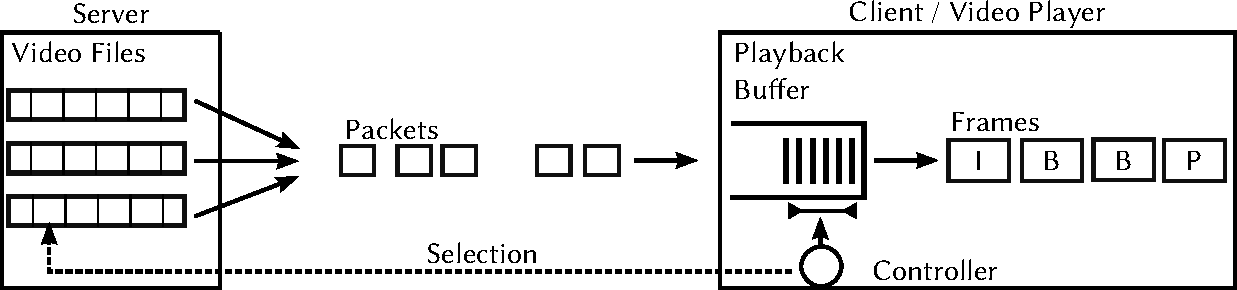
\includegraphics[width=0.9\textwidth]{images/playback-model.pdf}
    \caption{Reliable streaming playback model based on buffer control.}
    \label{c3:fig:playback-model}
\end{figure}

Figure~\ref{c3:fig:playback-model} overviews the reliable streaming model. The controller, part of the video player, selects a video from a remote location and the transmission is started, filling the playback buffer. The model has three degrees of freedom, which are all governed by the controller and together are coined playback strategies. These are:

\begin{itemize}
    \item The initial playback delay, which is the time between the initiation of the video stream transmission and the actual stream playback. The larger this is chosen, the bigger the safety margin on the buffer gets. If the video and transmission bitrate are known to be constant and and appropriately dimensioned, the initial delay can be chosen to be very small.
    \item Playback pause and resume decisions based on the current buffer fill level. This is a generalization of the initial playback delay, which is in fact only one, albeit always occurring stalling period.
    \item Selection of the video or video segment with a video bitrate chosen according to the current network throughput. This is only applicable for adaptive streaming.
\end{itemize}


These decisions yield a stalling period distribution for a streamed video. The frequency and the duration of stalls directly relate to the decision function of the playback model. The more frequent the stalls are, the shorter they will be; if the strategy produces longer stalls, they will be less frequent assuming the same network conditions. The time scale on which streaming applications buffer content usually lies in the range of seconds. This is a necessity in best-effort networks, as the available network bitrate might drop unexpectedly and cause stalling.


The the rest of this sections present fundamental playback strategies and strategy building blocks with features extracted from real world examples, which are given afterwards. 



%%
\subsubsection{Null Strategy}

The simplest strategy is having no strategy at all. Playback is started immediately when at least a single frame fully resides within the buffer and stops again at an empty buffer. The behavior can be summarized as ``Whenever anything can be played from the buffer, do so''.

This results in frequent stops and a large loss in playback continuity and will therefore not be used in practice. However, this strategy has some interesting theoretical properties, which is why it is mentioned here.
It minimizes total stalling time and the required buffer space. Moreover, it gives an upper limit for the number of stalls occurring\footnote{As a video frame is atomic, no other model could possibly stop the playback more often.}. Therefore, it can act as a baseline reference to assess the performance of other strategies.

\begin{figure}[htb]
    \centering
    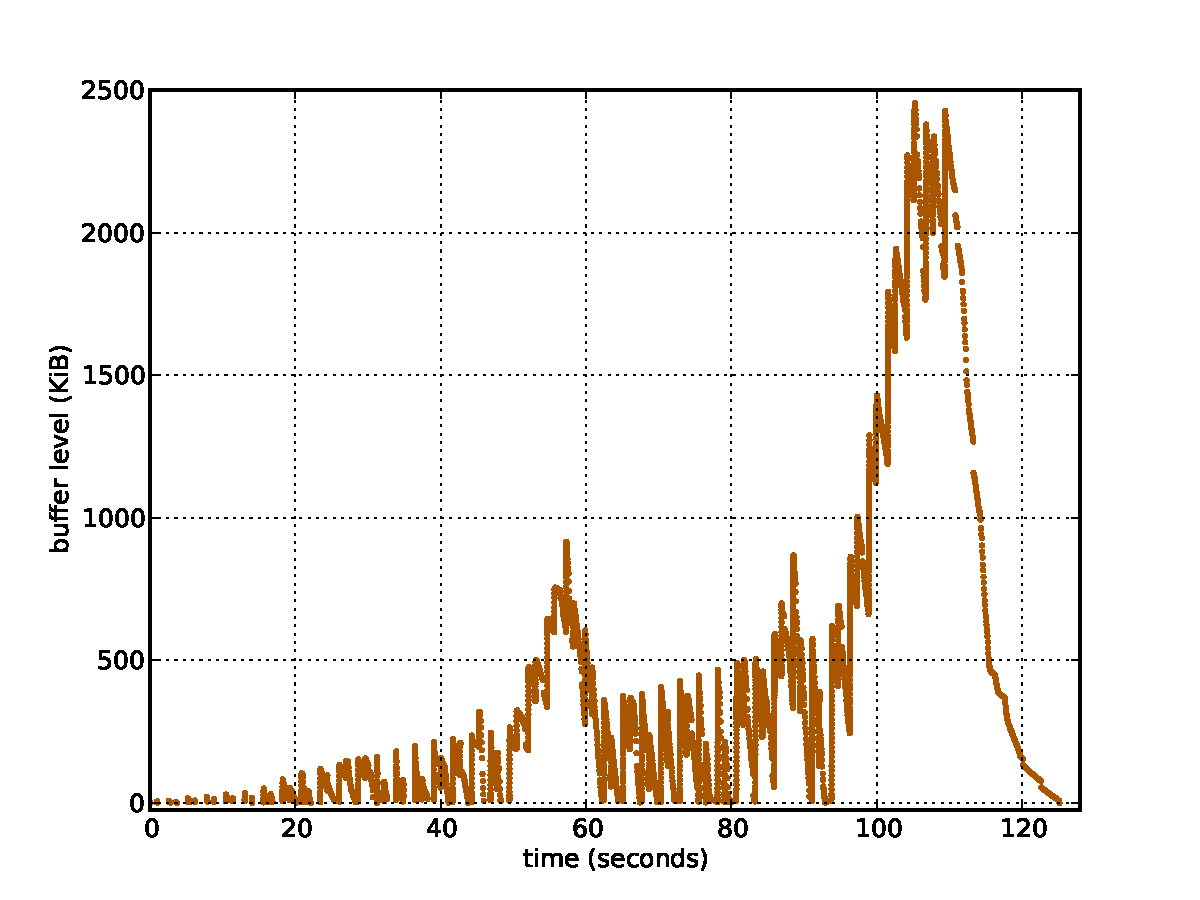
\includegraphics[width=0.9\textwidth]{images/bufferlevel-stall-new.pdf}
    \caption{Buffer fill level with null strategy; \SI{33}{\second} total stalling.}
    \label{c3:fig:bufferlevel-stall}
\end{figure}

Figure~\ref{c3:fig:bufferlevel-stall} depicts an exemplary time series diagram of the contents of a video buffer using this strategy with a transmission rate only slightly above the video stream's rate. The buffer frequently drops down to zero forcing a short stall. According to the presented related work on the \gls{QoE} impact of stalling frequency in comparison to the length of stalls \cite{6123395}, this is the worst possible scenario for a person watching the stream.


%%
\subsubsection{Threshold Strategies}

Instead of instantly restarting playback, a lower threshold can be introduced. Only after a certain buffer fill level threshold has been surpassed, playback will be started. Thresholds can be set independently for the initial playback delay and stalls, with the initial playback delay generally set to be higher.

The threshold can be chosen in a number of ways. It can either be an absolute data volume, a buffered video duration. The latter is much more suited for variable bitrate videos as it automatically adapts itself to the current bitrate. A third option is to buffer for a certain amount of real time -- this can be seen as threshold -- and starting playback after that period regardless of the volume of the buffer. Additionally, the threshold could also either be set to a constant value or dynamically chosen according to the expected network \gls{QoS}.

Besides this single-threshold strategy, a two-threshold strategy might make more sense for segment-based streaming. In addition to the lower threshold, an upper threshold is introduced. When reached, no new segments will be requested until the buffer arrives at the lower threshold again.  To achieve an hysteresis effect a third threshold, somewhere between the lower and upper bound, can also be introduced. Through this, the maximum buffer size can also be controlled. This is important in situations with hard limits on available memory. Mobile devices come to mind here.

\begin{figure}[htb]
    \centering
    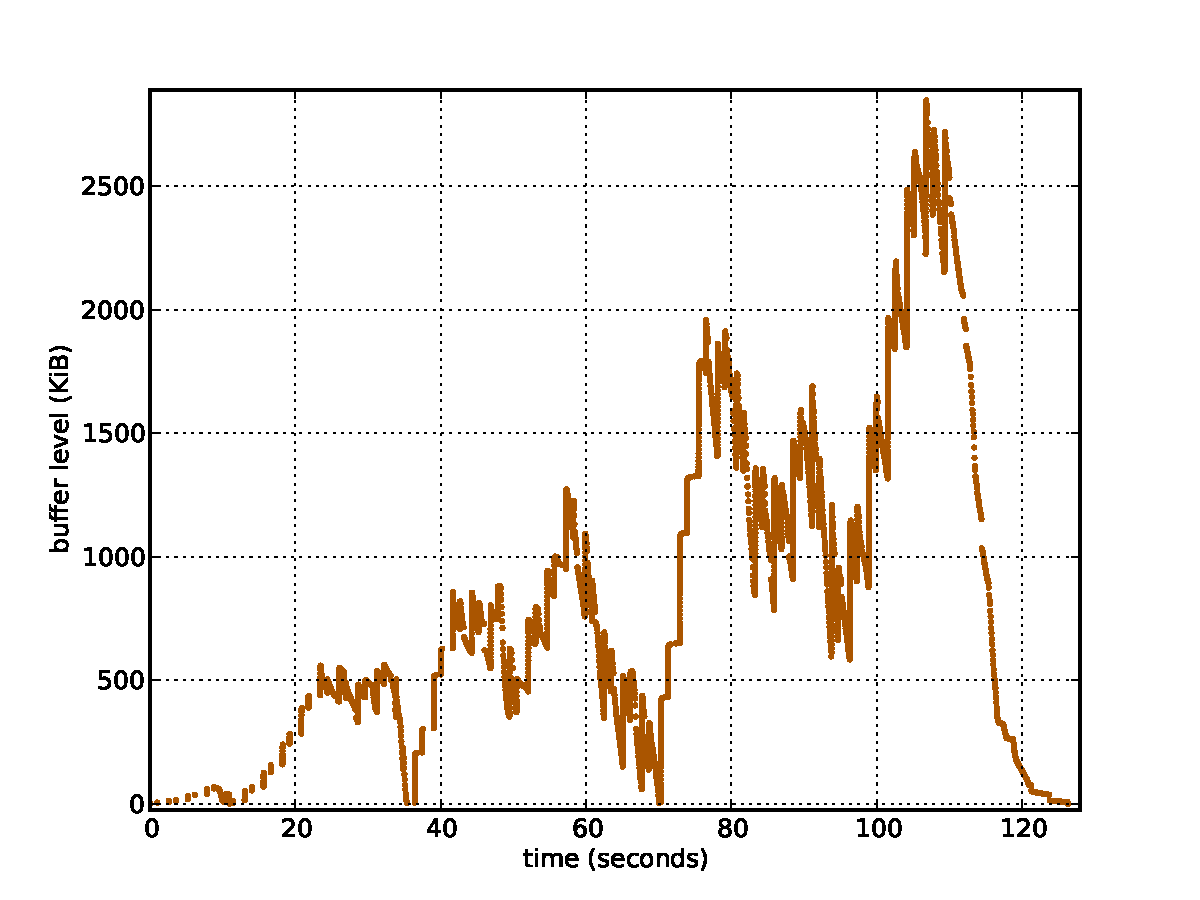
\includegraphics[width=0.9\textwidth]{images/bufferlevel-flash-new.pdf}
    \caption{Sample buffer fill level for a \SI{2}{\second} and \SI{5}{\second} buffered video duration threshold strategy; \SI{34}{\second} total stalling.}
    \label{c3:fig:bufferlevel-flash}
\end{figure}

An example buffer diagram is displayed in Figure~\ref{c3:fig:bufferlevel-flash}. In this case, the initial delay was controlled by a buffered video duration threshold of \SI{2}{\second} and a resume condition also based on buffered video duration but with a \SI{5}{\second} threshold. The strategy produces noticeable less stalls than the null strategy but slightly increases the total stalling time.


%%
\subsubsection{Pacing Strategies}

For segment-based \gls{HTTP} streaming, a two-threshold strategy is not the only supplemental option on top of simple streaming. Here, the controller can pace the request of future segments to match the overall, or the current video bitrate. A safety margin can also be factored in to even out short time fluctuations of either the transmission or the video bitrate. For example, the controller would request segments with an overall transmission rate of 1.25 times the video bitrate. The pacing rate can either be statically chosen in advance or can be calculated dynamically based on current or future conditions. The latter leads to predictive strategies.

%%
\subsubsection{Predictive Strategies}

In predictive strategies, knowledge of the future of the streaming process is used by the controller to adjust the start/stop and segment retrieval conditions. Instead of global knowledge, heuristics can instead attempt to approximate a future state.

A very simple predictive approach is to prolong the initial delay to the point, that no intermediate buffer underrun and thus no stall will occur. With global knowledge, the controller can start the stream at the earliest possible point in time, thus minimizing the total stalling time while still having only the initial delay.

\begin{figure}[htb]
    \centering
    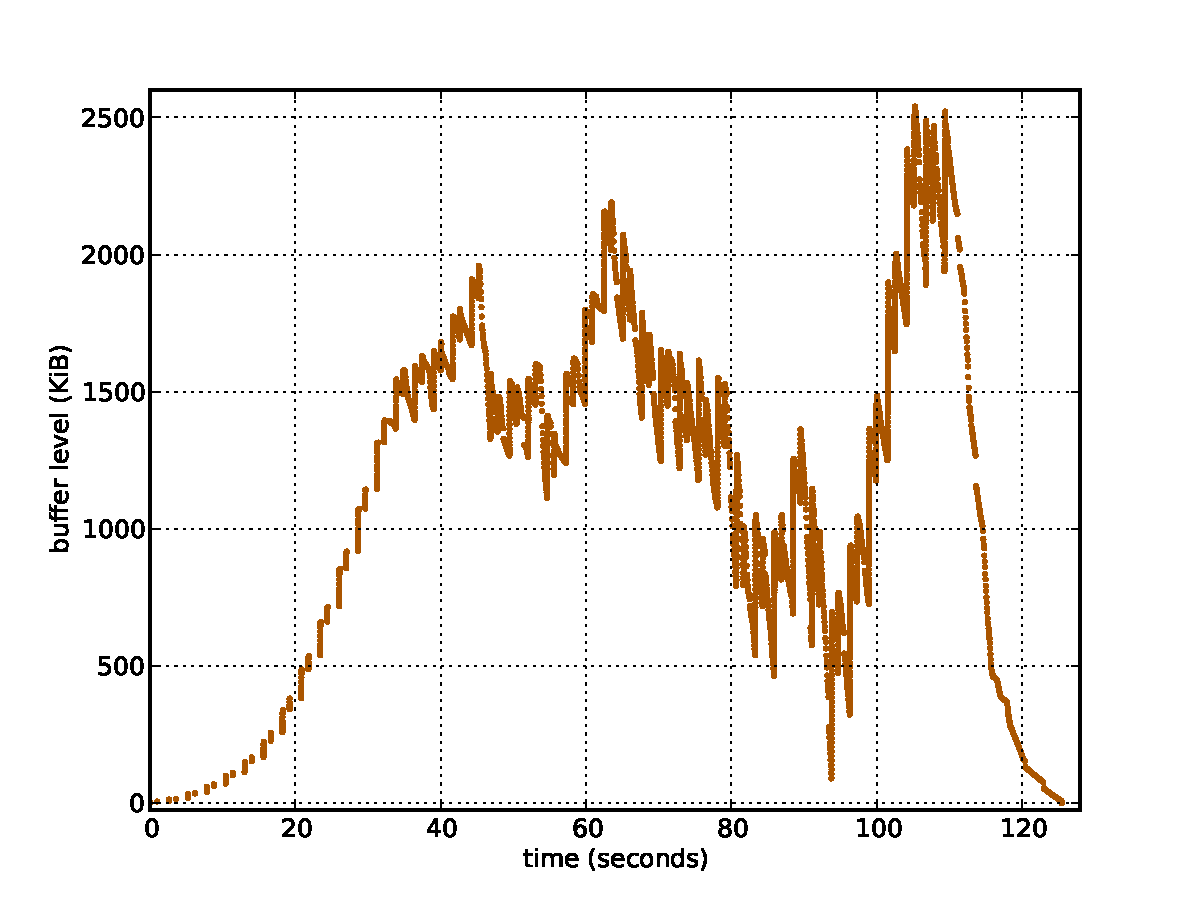
\includegraphics[width=0.9\textwidth]{images/bufferlevel-startdelay-new.pdf}
    \caption{Sample Buffer fill level for the delayed playback model, \SI{33}{\second} total stalling.}
    \label{c3:fig:bufferlevel-startdelay}
\end{figure}

Figure~\ref{c3:fig:bufferlevel-startdelay} depicts the time series of a sample implementation of this delayed playback predictive strategy with all necessary stalling occurring upfront.


%%
\subsubsection{Adaptive Strategies}

Most strategies for adaptive streaming are an extension of both the threshold as well as the pacing strategy. However, instead of a simple transmit-or-no-transmit ruleset, they can make much more fine-grained adjustments. The quality of the stream segment to be requested will be chosen, depending on the current fill level and drain rate of the buffer. This makes a trade off between maintaining a certain quality level and putting up with increased waiting times, and dropping the quality to a level sustainable at the current transmission rate.


\subsubsection{Real World Implementation Examples}

Actual streaming player implementations often do not implement only one of these strategies, but rather combine ideas from several. Herein, thresholds are often set arbitrarily through the implementor's best practices and not empirically evaluated, often making a trade-off between user perceivable quality and resulting server load. In general, every streaming service practically implements its own playback strategies. This section describes three example applications.

%%
\paragraph{2011 YouTube Flash Player Buffering Strategy}

Google's video streaming site YouTube is constantly changing its appearance and technical makeup. In recent years, YouTube streams are delivered by one of three players: The Website's Flash player, a browser-integrated HTML5-based player, or custom player implementations in mobile phones, set-top boxes and similar devices. Here, the Flash-based variant used in 2011 is described.

This player used a single threshold strategy with different threshold values for the initial delay and any subsequent stalls. The values were already described in Figure~\ref{c3:fig:bufferlevel-flash}. This model assumes sufficient network conditions in the beginning, requiring only a short initial playback delay to pre-fill the playback buffer. If, however, stalling occurs, then it will buffer longer to keep the stalling frequency down.

\begin{table}[htb]
    % increase table row spacing, adjust to taste
    %\renewcommand{\arraystretch}{1.3}
    \caption{Transmission Related Parameters from YouTube's Video URL Setup}
    \label{c3:tbl:yturl}
    \centering
    \begin{tabu}{|X[l]|X[p]|}
        \hline
        URL Part & Description \\ \hline
        \texttt{v$\alpha$.lscache$\beta$.c.youtube.com} &  Cache server involved in the delivery.\\
        \texttt{algorithm=throttle-factor} and \texttt{burst=40} and \texttt{factor=1.25} & Indicates initial burst plus block sending configuration. \\
        \texttt{ratebypass=yes} & Parameter to indicate no rate limiting.\\ \hline
    \end{tabu}
\end{table}

Furthermore, YouTube employs a proprietary pacing mechanism outside of the control of the streaming player. This is hinted at in the encoding of the \glspl{URL} of the video files and enforced by the video file cache server. Some of those not user-changeable parameters are described in Table~\ref{c3:tbl:yturl}. The pacing was in effect for all videos below high definition resolution, but has since then been extended to include all video files. 

\begin{figure}[htbp]
% used yt-delay/hPUGNCIozp0_delay_100 2, spyder with matplotlib config patch
    \centering
        \begin{subfigure}[b]{0.90\textwidth}
                \centering
                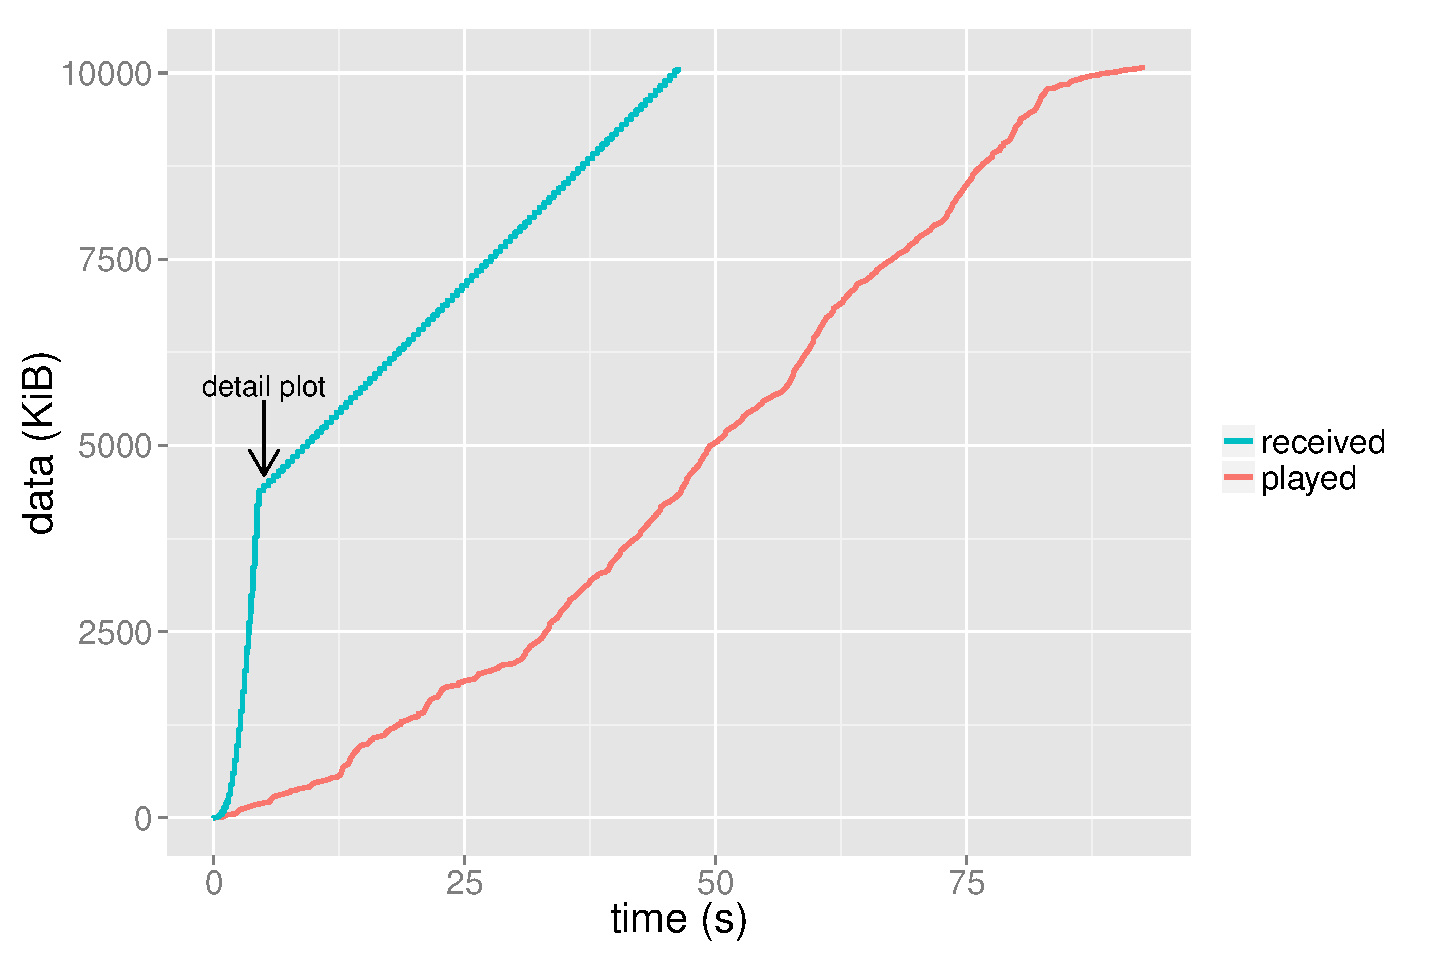
\includegraphics[width=\textwidth]{images/R-blocktransfer.pdf}
                \caption{Overall graph.}
                \label{c3:fig:blocktransfer-overall}
        \end{subfigure}

        \begin{subfigure}[b]{0.90\textwidth}
                \centering
                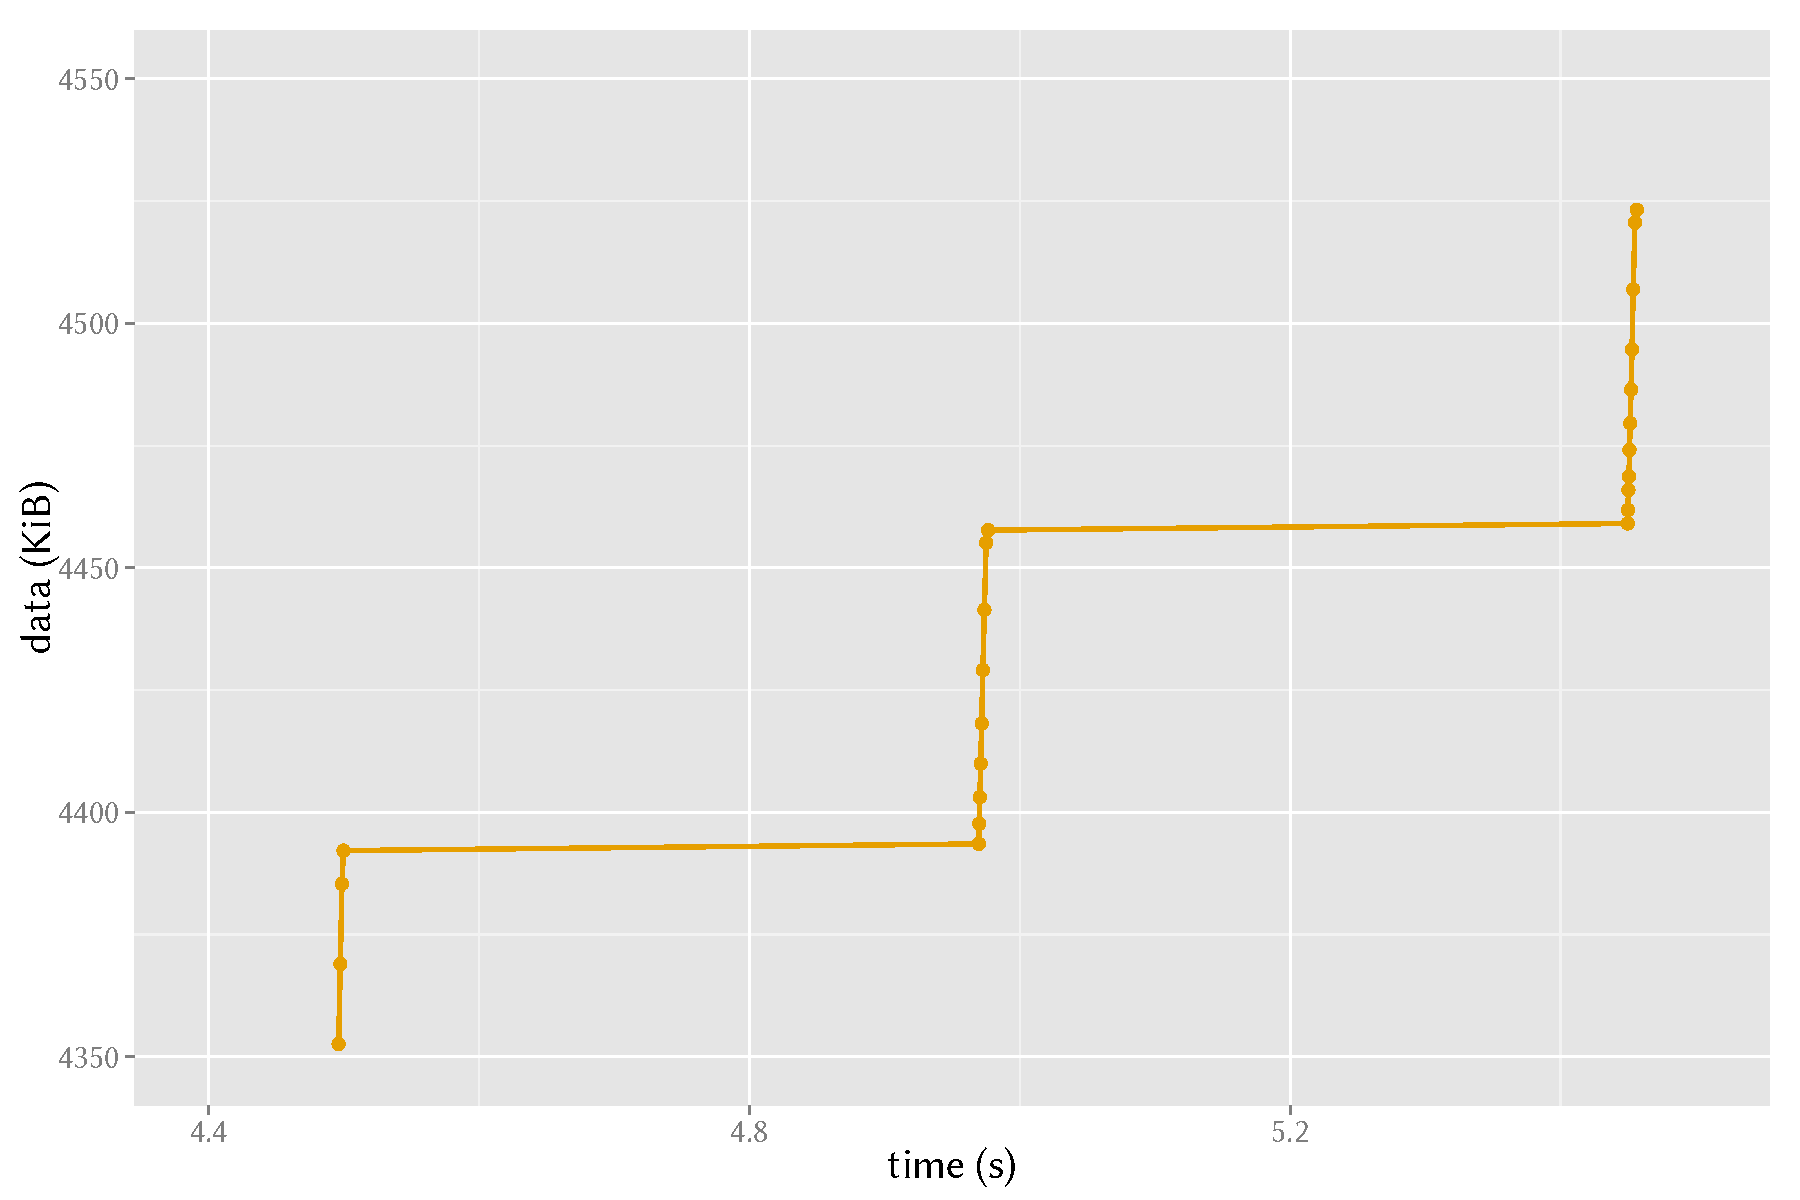
\includegraphics[width=\textwidth]{images/R-blocktransferdetail.pdf}
                \caption{Detail plot of the rate-limited block-sending phase.}
                \label{c3:fig:blocktransfer-detail}
        \end{subfigure}
\caption{Comparison of downloaded and consumed data volume revealing the pacing mechanism used by YouTube.}
\label{c3:fig:blocktransfer}
\end{figure}


The throttling method, also observed in \cite{alcock2011afcyt}, limits the transmission to a rate slightly above the average media bitrate, measurements and the \gls{URL} scheme indicates this to be a factor of the video bitrate of $1.25$. The rate limit is not constant, instead a ON-OFF block-sending scheme is facilitated. The scheme transmits short packet bursts, typically \SI{64}{\kibi\byte} in size, followed by long pauses as seen in Figure~\ref{c3:fig:blocktransfer}. The pause length between two bursts is set dynamically to reach the targeted bitrate on a larger time scale. The initial phase of the stream transmission is conducted unthrottled at line speed, presumably to allow for some pre-buffering to occur at the client media player. A possible reason for this server-side pacing is to avoid load spikes, with the added side effect of keeping the clients' buffer sizes in check.



%%
\paragraph{Firefox's HTML5 Player Strategy}

Video streaming can also be directly conducted with the Web browser, through the use of a HTML5 canvas element. The \gls{W3C} specifies the default technical process of HTMl5 video streaming in \cite{html5video} and essentially suggests a predictive strategy. Herein, the Web browser should estimate and correlate the transmission rate to the video bitrate. A property called ``autoplay'' uses this definition to start  playback of the associated video \enquote{as soon as it can do so without stopping}. The HTML5 strategy also allows to limit the buffer size through transmission pacing, negotiated with the server, and appropriately timed range requests.

The open-source Firefox browser represents an implementation of this specification and substantiates it further. The description of this strategy is based on Firefox's version 4.0 released in March 2011. Because it is an online algorithm which does not have global knowledge of the video and transmission speeds of any point in the future it has to estimate these.
To estimate the current and future rates, the moving average of the transmission rate $s_{MA}$ and the video bitrate $v_{MA}$ are calculated. The condition $c$ Firefox uses to start and resume the playback process is given in Algorithm~\ref{c3:alg:firefox}, with the buffered video duration $b_b$, and the duration spent buffering $b_T$.

\begin{algorithm}[htb]
    \centering
    \begin{algorithmic}
        \IF {$s_{MA} > v_{MA}$} 
          \STATE $c \gets ( b_b=20s \lor b_T=20s )$
        \ELSE
          \STATE $c \gets ( b_b=30s \lor b_T=30s )$
        \ENDIF 
    \end{algorithmic}
    \caption{Firefox playback (re-)start decision algorithm.}
    \label{c3:alg:firefox}
\end{algorithm}

 \begin{figure}[htb]
    \centering
    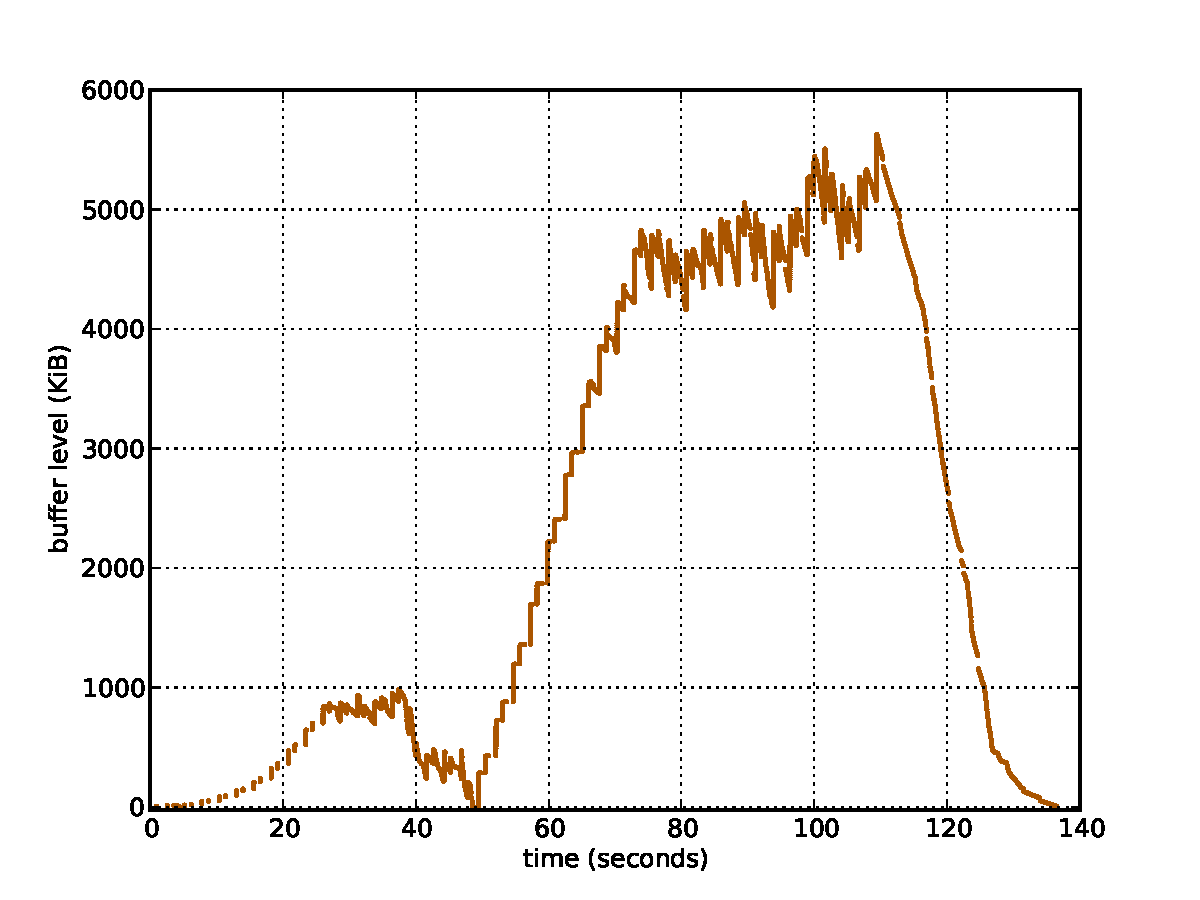
\includegraphics[width=0.9\textwidth]{images/bufferlevel-firefox-new.pdf}
    \caption{Sample buffer fill level for the Firefox 4 strategy, \SI{44}{\second} total stalling.}
    \label{c3:fig:bufferlevel-firefox}
\end{figure}


This approach is quite conservative and trades off long stalling periods for fewer stalls. The test case for our model is shown in Figure \ref{c3:fig:bufferlevel-firefox}. The playback starts only after a long waiting period and intermittent stalls cause a long buffering period. 
Due to the longer overall stalling time the player needs to buffer more data than other strategies. This may make it unsuitable for devices with sparse amounts of memory, e.g. mobile phones. On the other hand, could a large buffer also increase the chance of continuous playback in such scenarios with bad \gls{QoS}.


\paragraph{Adaptive streaming strategies}

Implementations for adaptive streaming players are again mostly proprietary and their behavior has to be derived from measurements. This is even true for adaptive streaming protocols, which have open specifications as these generally do not specify the player's behavior.

Microsoft's Silverlight player's strategy is described in \cite{BLTJ:BLTJ20505}. It employs a two-threshold model and rate estimations. When on of the thresholds is reached, the quality will be adjusted by one step upwards or downwards as long as the transmission rate is sufficient.

The buffering behavior of further protocol variants, including Adobe's \gls{HTTP} Dynamic Streaming, Apple's \gls{HTTP} Live Streaming and a sample implementation of \gls{DASH}, are investigated in \cite{Muller:2012:EDA:2151677.2151686,akhshabi2011experimental}.




% \begin{itemize}
% \item The player has been buffering data for at least 30 seconds.
% \item The player has already buffered an amount of data corresponding to 30 seconds of video.
% \item The video download has been completed.
% \item The moving average of the transmission rate is larger than the moving average of the video bitrate and the player has a safety buffer with 20 seconds of video data.
% \end{itemize}

% \begin{table}[htb]
%     \caption{Variables involved in buffering decisions.}
%     \label{c3:tbl:buffvars}
%     \centering
%     \begin{tabu}{|l|X[p]|} 
%     \hline
%     Variable & Description \\ \hline
%     $s_{MA}$ & Moving average of the transmission speed. \\
%     $v_{MA}$ & Moving average of the video bitrate. \\ 
%     $c$   & Condition upon which to start/resume playback. \\
%     $b_b$    & Amount of video data the buffer contains. \\
%     $b_T$    & Amount of time spent in non-playing buffering state. \\ \hline
%     \end{tabu}
% \end{table}

% used yt-delay/hPUGNCIozp0_delay_2500 1, spyder, color #aa5500
% data
% start delay 33s 
% flash 33.82s
% stalling 32.68s
% html5 as implemented in firefox 44s


%Which offers better quality to users? Some approaches (TODO: refs and explain how)

% Longer waiting time but very few stops. Stalling model definitely the shortest waiting time but stops too frequent with insufficient network conditions, i.e. can not really be used. Delayed playback requires total knowledge not available beforehand. Can maybe used with reduced information, bandwidth estimation, but this is essentially HTML5/Firefox.




%``application comfort'' time to skip, ...
%\subsubsection{Unreliable Streaming Metrics}
%... and why they mostly do not work / are not applicable.